\documentclass[12pt,a4paper]{article}
\usepackage[utf8]{inputenc}
\usepackage[spanish,es-tabla]{babel}
\usepackage[T1]{fontenc}
\usepackage{times}
\usepackage{geometry}
\geometry{
  top=4.2cm,
  bottom=2.5cm,
  left=3.0cm,
  right=3.0cm,
  headheight=95pt,
  headsep=15pt,
  footskip=1.0cm
}

\usepackage{graphicx}
\usepackage{fancyhdr}
\usepackage{enumitem}
\usepackage{tabularx}
\usepackage{array}
\usepackage{float}
\usepackage{amssymb}
\usepackage{xcolor}

% Configuración del encabezado institucional idéntico al documento Word
\pagestyle{fancy}
\fancyhf{}
\renewcommand{\headrulewidth}{0pt}
\fancyhead[C]{%
  \begin{minipage}[c]{0.14\textwidth}
    \raggedright
    
\includegraphics[height=1.85cm,keepaspectratio]{image3.png}
  \end{minipage}%
  \hfill
  \begin{minipage}[c]{0.70\textwidth}
    \centering
    {\fontsize{11}{13}\selectfont\textbf{UNIVERSIDAD TÉCNICA DE AMBATO}}\\[2pt]
    {\fontsize{9}{11}\selectfont\textbf{FACULTAD DE INGENIERÍA EN SISTEMAS ELECTRÓNICA E INDUSTRIAL}}\\[2pt]
    {\fontsize{9}{11}\selectfont\textbf{CARRERA DE SOFTWARE}}\\[3pt]
    \noindent\rule{\linewidth}{1pt}\\[3pt]
    {\fontsize{8.5}{10.5}\selectfont\textbf{CICLO ACADÉMICO: JULIO 2026 – DICIEMBRE 2026}}
  \end{minipage}%
  \hfill
  \begin{minipage}[c]{0.14\textwidth}
    \raggedleft
    
\includegraphics[height=1.85cm,keepaspectratio]{image2.png}
  \end{minipage}%
}

\setlength{\parindent}{0pt}
\setlength{\parskip}{5pt}

\begin{document}

\begin{center}
  \textbf{\underline{\large INFORME DE GUÍA PRÁCTICA 4}}
\end{center}

\vspace{0.3cm}

\noindent\textbf{I. PORTADA}

\vspace{0.2cm}

\noindent
\begin{tabular}{@{}p{6.0cm}p{8.8cm}@{}}
  \textbf{Tema:} & Construcción e integración de una arquitectura multicanal de vehículos, compradores, ventas y notificaciones. \\[5pt]
  \textbf{Unidad de Organización Curricular:} & PROFESIONAL \\[5pt]
  \textbf{Nivel y Paralelo:} & 5to “B” \\[5pt]
  \textbf{Alumnos participantes:} & De la Cruz Llundo Carolina Elizabeth \\[5pt]
  \textbf{Asignatura:} & APLICACIONES ORIENTADAS A SERVICIOS \\[5pt]
  \textbf{Docente:} & Ing. Javier Vargas, Mg.
\end{tabular}

\vspace{0.4cm}

\noindent\textbf{II. INFORME DE GUÍA PRÁCTICA}

\vspace{0.2cm}

\noindent\textbf{1.1 Objetivos}

\vspace{0.1cm}

\noindent\textbf{General:}

\noindent Integrar aplicaciones de escritorio, web y móvil con una arquitectura de servicios REST basada en Java Spring Boot y Python FastAPI, manteniendo autenticación JWT, balanceo de carga con NGINX, persistencia MySQL y comunicación asíncrona mediante RabbitMQ para ejecutar ventas desde una PWA y visualizar sus notificaciones en JavaFX.

\vspace{0.1cm}

\noindent\textbf{Específicos:}

\begin{itemize}[leftmargin=*,itemsep=2pt,topsep=2pt]
  \item Adaptar, ampliar y verificar los proyectos base y sus servicios REST para cumplir la arquitectura y los contratos funcionales exigidos, manteniendo en el backend las responsabilidades de negocio y seguridad.
  \item Implementar las funciones administrativas de Windows Forms, el flujo autenticado de venta desde PWA y las consultas de React.
  \item Integrar la publicación y consumo de eventos de venta mediante RabbitMQ y presentar las notificaciones en JavaFX.
  \item Mantener dos instancias de la API Java detrás de NGINX y comprobar la disponibilidad, la seguridad y la continuidad de las solicitudes.
  \item Demostrar el funcionamiento extremo a extremo mediante código ejecutable, registros, resultados HTTP, evidencias visuales y pruebas de recuperación.
\end{itemize}

\vspace{0.2cm}

\noindent\textbf{1.2 Modalidad}

\noindent Presencial.

\vspace{0.2cm}

\noindent\textbf{1.3 Tiempo de duración}

\noindent\textbf{Presenciales:} 12\\
\textbf{No presenciales:} 0

\vspace{0.2cm}

\noindent\textbf{1.4 Instrucciones}

\noindent La arquitectura de referencia define el resultado funcional esperado. Cada estudiante podrá adaptar los proyectos base y su configuración para implementar los cuatro clientes, NGINX, los servicios REST, RabbitMQ y la persistencia.

\begin{figure}[H]
  \centering
  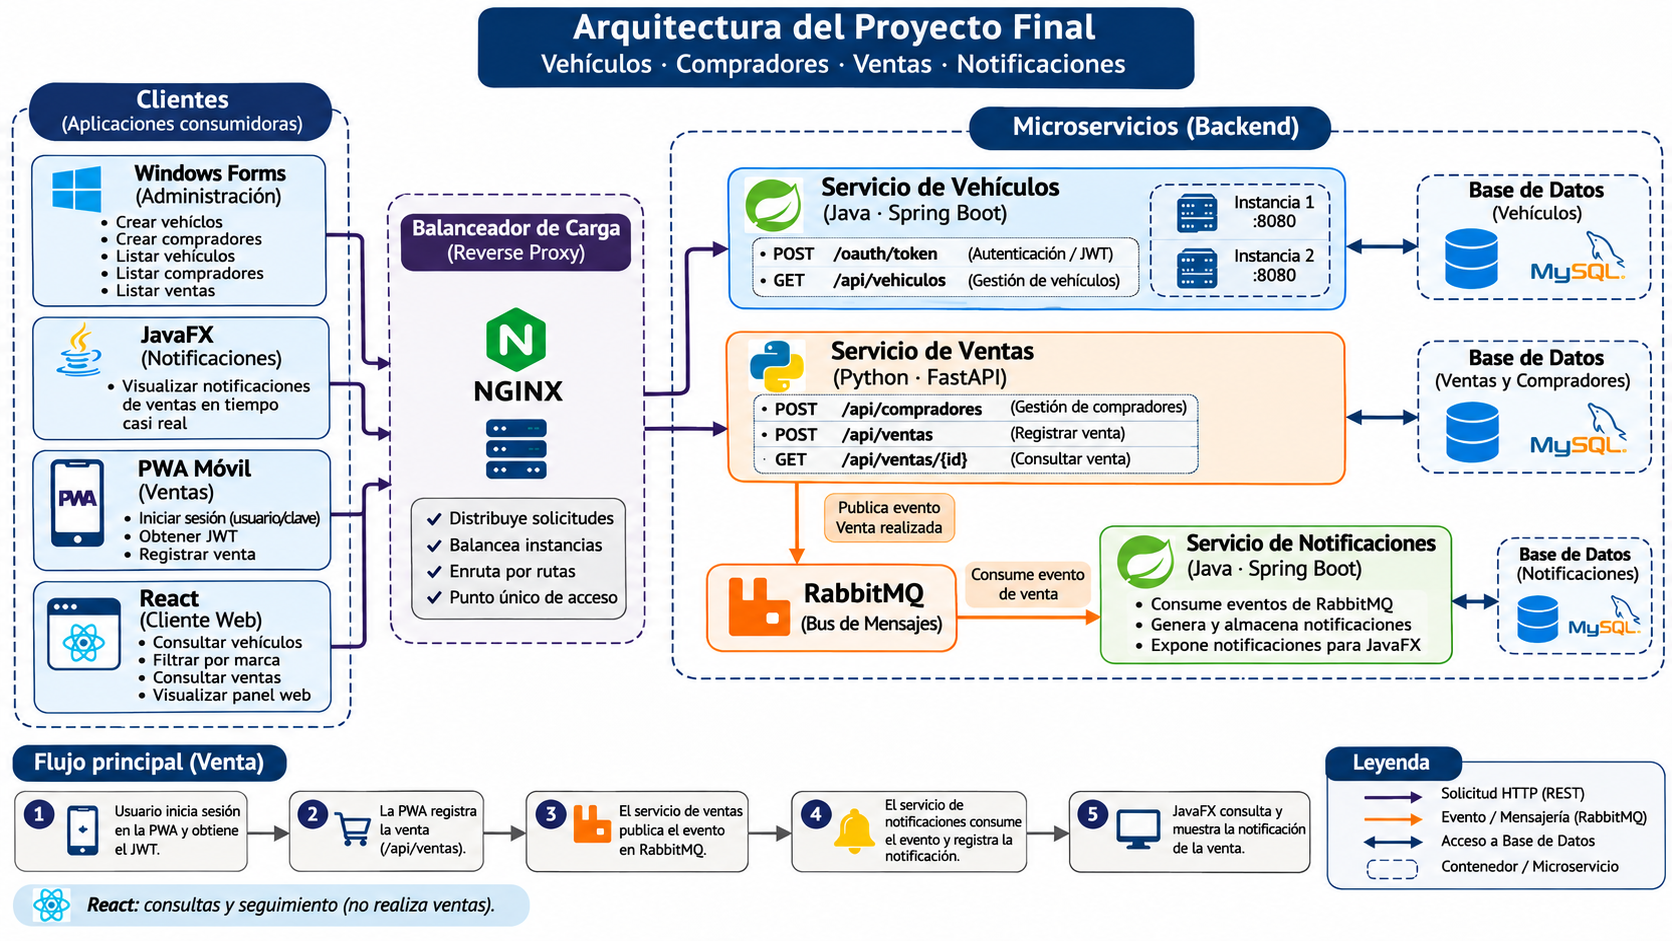
\includegraphics[width=\textwidth]{image1.png}
\end{figure}

\noindent La arquitectura es conceptual y establece responsabilidades obligatorias. Se podrán realizar ajustes técnicos justificados en los proyectos base para obtener una implementación equivalente, funcional y verificable. Se conservan como referencia las instancias Java 8080/8082 y se identifican los endpoints por incorporar.

\vspace{0.2cm}

\noindent\textbf{Caso y alcance funcional:}

\noindent Una operación comercial requiere registrar vehículos y compradores desde una aplicación administrativa, consultar los datos desde una plataforma web, autenticar a quien realiza la venta desde una aplicación móvil y notificar automáticamente la operación a una aplicación JavaFX. Todos los clientes utilizarán servicios compartidos, con acceso controlado mediante JWT. Los eventos de negocio circularán por RabbitMQ y los datos persistirán exclusivamente en las bases de datos de los servicios.

\noindent MODIFICACIONES PERMITIDAS: La solución no exige conservar intactos los proyectos base. Se puede modificar libremente sus componentes técnicos, interfaces, código fuente, endpoints y configuraciones, así como incorporar módulos adicionales, siempre que la implementación final cumpla todos los requerimientos y sus pruebas sean reproducibles.

\vspace{0.2cm}

\noindent\textbf{Responsabilidad obligatoria de cada aplicación}

\vspace{0.1cm}

\noindent
\begin{tabularx}{\textwidth}{|>{\bfseries\raggedright\arraybackslash}p{4.2cm}|X|}
\hline
Componente & Funciones exigidas \\
\hline
Windows Forms $\cdot$ C\# / .NET 8 & Crear vehículos; crear compradores; listar vehículos, compradores y ventas. Mostrar códigos HTTP y errores del servicio. \\
\hline
PWA móvil $\cdot$ HTML/CSS/JavaScript & Iniciar sesión con usuario y contraseña; obtener JWT mediante /oauth/token; consultar datos necesarios; registrar ventas y consultar su estado. \\
\hline
React $\cdot$ Vite + Fetch & Consultar vehículos; filtrar por marca; consultar ventas y visualizar resultados o indicadores sustentados en información real. No registrar ventas. \\
\hline
JavaFX $\cdot$ Java & Consultar o recibir notificaciones de venta y mostrarlas en pantalla, actualizando el estado sin intervención manual reiterada. \\
\hline
API de vehículos $\cdot$ Java Spring Boot & Autenticación y autorización JWT; operaciones de vehículos; dos instancias equivalentes detrás de NGINX. \\
\hline
API de ventas $\cdot$ Python FastAPI & Operaciones de compradores y ventas, validaciones e idempotencia; publicación de evento después de confirmar una venta. \\
\hline
Notificaciones $\cdot$ Spring Boot & Consumir RabbitMQ, registrar notificaciones y exponer un canal de consulta/actualización para JavaFX. \\
\hline
NGINX, RabbitMQ y MySQL & Enrutamiento y balanceo; transporte persistente de eventos; persistencia de los datos con responsabilidades separadas. \\
\hline
\end{tabularx}

\vspace{0.3cm}

\noindent\textbf{Alcance de modificación de proyectos base y restricciones técnicas:}

\begin{itemize}[leftmargin=*,itemsep=2pt,topsep=2pt]
  \item Se permite modificar, ampliar, refactorizar y reorganizar TODOS los proyectos base disponibles: servicio Java de vehículos, servicio Python de compradores/ventas, servicio Java de notificaciones, Windows Forms, JavaFX, React y PWA móvil. También podrán adaptarse NGINX, RabbitMQ, las migraciones SQL y las configuraciones de integración. Se pueden crear o cambiar clases, controladores, servicios, repositorios, DTO, rutas, dependencias, formularios, vistas y mecanismos de comunicación que sean necesarios para lograr el funcionamiento solicitado.
  \item Las modificaciones están autorizadas siempre que se mantengan los resultados funcionales exigidos, las validaciones, la seguridad JWT, la autorización, la idempotencia y la persistencia coherente. No se trasladarán al frontend reglas de negocio que deban ejecutarse en los servicios. La PWA será el único cliente con funcionalidad de registro de ventas; Windows Forms y React consultarán ventas. Esta exclusividad deberá comprobarse en las interfaces y en el control de permisos del backend.
  \item Las credenciales se ingresarán en el formulario de login móvil. El JWT deberá provenir de esa autenticación y no de un token copiado manualmente desde Postman para ejecutar una venta.
  \item Las API no compartirán acceso directo a tablas ajenas. Se permite un único servidor MySQL con esquemas lógicos separados, siempre que se mantengan las responsabilidades por servicio.
  \item No se codificarán contraseñas, claves JWT, secretos de integración ni URL internas sensibles en el repositorio. Se utilizarán variables de entorno o configuraciones locales excluidas de Git.
  \item La aplicación JavaFX no accederá directamente a RabbitMQ ni a MySQL: utilizará un endpoint o canal expuesto por el servicio de notificaciones.
  \item Se mantendrá NGINX como puerta de entrada para peticiones REST. El monitor de balanceo podrá seguir funcionando de forma independiente, sin ubicarse en el flujo obligatorio de las transacciones.
\end{itemize}

\vspace{0.2cm}

\noindent\textbf{Contrato mínimo de servicios:}

\vspace{0.1cm}

\noindent
\begin{tabularx}{\textwidth}{|>{\raggedright\arraybackslash}p{4.5cm}|>{\raggedright\arraybackslash}p{3.8cm}|X|}
\hline
\textbf{Método y ruta} & \textbf{Servicio} & \textbf{Condición} \\
\hline
POST /oauth/token & Vehículos / autenticación & Existente; autentica y emite JWT. \\
\hline
GET /api/vehiculos & Vehículos & Existente; catálogo autorizado. \\
\hline
POST /api/vehiculos & Vehículos & Verificar el contrato actual; conservar o completar la operación administrativa sin alterar reglas. \\
\hline
POST /api/compradores & Ventas / compradores & Existente; registrar comprador. \\
\hline
GET /api/compradores & Ventas / compradores & Incorporar si aún no existe; listar compradores autorizados. \\
\hline
POST /api/ventas & Ventas & Existente; registrar venta con Idempotency-Key. \\
\hline
GET /api/ventas/\{id\} & Ventas & Existente; consultar estado individual. \\
\hline
GET /api/ventas & Ventas & Incorporar si aún no existe; listado administrativo y consulta web. \\
\hline
GET /api/notificaciones & Notificaciones & Incorporar o utilizar ruta equivalente; consultar historial para JavaFX. \\
\hline
GET /api/notificaciones/stream & Notificaciones & Alternativa opcional a polling: SSE o WebSocket documentado. \\
\hline
\end{tabularx}

\vspace{0.3cm}

\noindent\textbf{1.5 Listado de equipos, materiales y recursos}

\vspace{0.1cm}

\noindent
\begin{tabularx}{\textwidth}{|>{\bfseries\raggedright\arraybackslash}p{5.5cm}|X|}
\hline
Herramienta / recurso & Uso mínimo \\
\hline
Windows 10/11 y VS Code / Visual Studio & Edición, compilación y ejecución de aplicaciones cliente. \\
\hline
JDK 17, Maven y JavaFX & Servicios Java y cliente JavaFX, manteniendo la versión efectiva del proyecto. \\
\hline
.NET SDK 8 y Visual Studio & Aplicación administrativa Windows Forms. \\
\hline
Python, pip y entorno virtual & Ejecución del servicio FastAPI y migraciones de su base. \\
\hline
Node.js y npm & Clientes React y PWA móvil en el navegador. \\
\hline
MySQL o XAMPP & Base de datos operativa de vehículos y ventas; almacenamiento de avisos cuando corresponda. \\
\hline
NGINX & Enrutamiento y balanceo hacia dos instancias Spring Boot. \\
\hline
RabbitMQ con interfaz de administración & Cola durable y verificación de mensajes pendientes y consumidos. \\
\hline
Postman, navegador y Git / GitHub & Pruebas HTTP, revisión de peticiones y trazabilidad de código. \\
\hline
\end{tabularx}

\vspace{0.3cm}

\noindent\textbf{Puertos de referencia:}

\vspace{0.1cm}

\noindent
\begin{tabularx}{\textwidth}{|>{\bfseries\raggedright\arraybackslash}p{4.2cm}|>{\centering\arraybackslash}p{2.6cm}|X|}
\hline
Componente & Puerto & Observación \\
\hline
NGINX & 8090 & Punto único de entrada REST en entorno local. \\
\hline
Vehículos A y B & 8080 / 8082 & Dos procesos equivalentes conectados a los mismos datos. \\
\hline
Ventas FastAPI & 8002 & Servicio de compradores y ventas. \\
\hline
Notificaciones & 8081 & API de consulta de avisos y consumidor RabbitMQ. \\
\hline
Monitor de NGINX & 8083 & Servicio de supervisión reutilizable y externo al flujo de venta. \\
\hline
RabbitMQ & 5672 / 15672 & AMQP y panel de administración, respectivamente. \\
\hline
MySQL & 3306 & Puerto habitual; verificar configuración local. \\
\hline
React / PWA en desarrollo & 5173 / 5174 & Se pueden usar puertos distintos al ejecutarse simultáneamente. \\
\hline
\end{tabularx}

\vspace{0.3cm}

\noindent TAC (Tecnologías para el Aprendizaje y Conocimiento) empleados en la guía práctica:

\begin{itemize}[label={},leftmargin=1.5em,itemsep=1pt,topsep=2pt]
  \item [$\boxtimes$] Plataformas educativas
  \item [$\square$] Simuladores y laboratorios virtuales
  \item [$\boxtimes$] Aplicaciones educativas
  \item [$\square$] Recursos audiovisuales
  \item [$\square$] Gamificación
  \item [$\boxtimes$] Inteligencia Artificial
\end{itemize}

\noindent Otros (Especifique): \underline{\hspace{6cm}}

\vspace{0.3cm}

\noindent\textbf{1.6 Actividades por desarrollar}

\vspace{0.2cm}

\noindent\textbf{Actividad 1. Diagnóstico inicial y definición de contratos}
\begin{itemize}[leftmargin=*,itemsep=2pt,topsep=2pt]
  \item Identificar los siete proyectos base y sus tecnologías; determinar los archivos, interfaces, endpoints, configuraciones y componentes que será necesario modificar, crear o reemplazar para completar la arquitectura.
  \item Comprobar que la API Java y FastAPI se conectan a MySQL; identificar DTO, Controller, Service, Repository y seguridad.
  \item Validar mediante Postman el login, la consulta de vehículos y las operaciones existentes de compradores y ventas. Registrar qué endpoints de listado requieren ampliación.
  \item Definir roles autorizados para escritura, consulta y venta; usar los roles reales del backend (CONSULTA, OPERADOR y ADMIN cuando correspondan).
\end{itemize}
\textbf{Evidencia mínima:} Matriz endpoint–método–rol–HTTP, estructura de proyectos y capturas de los servicios ejecutándose con respuestas reales.

\vspace{0.2cm}

\noindent\textbf{Actividad 2. Preparación de proyectos, configuración y control de versiones}
\begin{itemize}[leftmargin=*,itemsep=2pt,topsep=2pt]
  \item Organizar los siete proyectos base en repositorios o directorios identificados. Se autoriza modificar todos sus archivos y componentes para cumplir la integración; conservar un README por proyecto con requisitos, configuración, compilación y ejecución.
  \item Registrar los cambios efectuados en cada proyecto y justificar su relación con el requisito funcional correspondiente. Separar configuraciones locales de secretos y publicar únicamente plantillas sin valores reales.
  \item Comprobar que los proyectos compilan y que no se incluyen node\_modules, target, bin, obj, .venv, .git ni archivos temporales.
\end{itemize}
\textbf{Evidencia mínima:} Capturas de estructura de carpetas, comandos de compilación y estados de control de versiones sin archivos sensibles.

\vspace{0.2cm}

\noindent\textbf{Actividad 3. Vehículos, JWT, NGINX y disponibilidad}
\begin{itemize}[leftmargin=*,itemsep=2pt,topsep=2pt]
  \item Mantener el servicio Spring Boot de vehículos en dos instancias: A (8080) y B (8082), compartiendo la misma configuración de validación JWT y base de datos.
  \item Configurar NGINX en el puerto 8090 para enrutar /oauth/token y /api/vehiculos hacia el upstream; conservar balanceo ponderado 3:1 y tolerancia a fallos, sin exigir 75/25 exacto en muestras pequeñas.
  \item Configurar rutas de entrada hacia FastAPI y notificaciones mediante proxy cuando corresponda, sin asumir que el balanceo de vehículos se aplica automáticamente a otros servicios.
  \item Comprobar la sintaxis de NGINX y el funcionamiento de /nginx-ping y /actuator/health; reutilizar el monitor de estados, estadísticas y alertas cuando esté disponible.
\end{itemize}
\textbf{Evidencia mínima:} Configuración nginx.conf, respuesta de las dos instancias, nginx -t, al menos 100 GET con conteos reales y una prueba de continuidad con una instancia detenida.

\vspace{0.2cm}

\noindent\textbf{Actividad 4. Servicio de compradores y ventas en Python FastAPI}
\begin{itemize}[leftmargin=*,itemsep=2pt,topsep=2pt]
  \item Conservar POST /api/compradores, POST /api/ventas y GET /api/ventas/\{id\}; añadir GET /api/compradores y GET /api/ventas únicamente si todavía no están implementados.
  \item Aplicar las validaciones comerciales y la autorización correspondientes a cada operación; FastAPI validará autenticidad, expiración y permisos del JWT de usuario recibido. No permitir que el precio ni el estado definitivo dependan solo del cliente.
  \item Preservar Idempotency-Key: mismo identificador y misma solicitud no deben generar dos ventas; clave repetida con cuerpo diferente debe rechazarse según el contrato.
  \item Confirmar cambios en la base de datos y el estado de la operación; evitar notificar ventas rechazadas o estados no confirmados.
\end{itemize}
\textbf{Evidencia mínima:} Código de endpoints, validaciones, operaciones SQL reales y respuestas de creación/consulta con identificación de venta e idempotencia.

\vspace{0.2cm}

\noindent\textbf{Actividad 5. Cliente Windows Forms de administración}
\begin{itemize}[leftmargin=*,itemsep=2pt,topsep=2pt]
  \item Ampliar el proyecto C\# .NET 8 para crear vehículos y compradores y listar vehículos, compradores y ventas en controles apropiados.
  \item Consumir la API Java para vehículos y el servicio Python para compradores/ventas mediante NGINX; utilizar métodos POST/GET y enviar JWT de usuario autorizado.
  \item Separar la comunicación HTTP del formulario; presentar carga, confirmaciones, errores de validación, 401, 403, 404 y errores de conexión.
  \item Evitar agregar botones o métodos de registro de ventas a Windows Forms.
\end{itemize}
\textbf{Evidencia mínima:} Capturas de las cinco operaciones, fragmentos del cliente HTTP y resultados coherentes con las API y las bases de datos.

\vspace{0.2cm}

\noindent\textbf{Actividad 6. PWA móvil con login y registro exclusivo de ventas}
\begin{itemize}[leftmargin=*,itemsep=2pt,topsep=2pt]
  \item Construir pantalla de inicio de sesión con usuario y contraseña. Enviar POST /oauth/token a través de NGINX y obtener un JWT emitido para esa cuenta.
  \item Conservar el token solo durante la sesión de prueba, sin incrustarlo en código, guardarlo en el repositorio ni incluirlo en capturas.
  \item Mostrar vehículos y compradores necesarios para la venta; seleccionar datos válidos y ejecutar POST /api/ventas con Authorization: Bearer JWT e Idempotency-Key.
  \item Mostrar el resultado real (201, 200, 202 u otro según el contrato), estado de venta y mensaje comprensible. Permitir consulta posterior GET /api/ventas/\{id\}, en especial ante una respuesta incierta.
  \item Preparar el manifiesto, íconos y comportamiento adaptable a móvil; verificar la instalación PWA sobre un origen seguro cuando corresponda.
\end{itemize}
\textbf{Evidencia mínima:} Pantallas de login, JWT obtenido en la sesión sin exponerlo, catálogo, formulario, confirmación/estado y registros HTTP de venta.

\vspace{0.2cm}

\noindent\textbf{Actividad 7. Cliente web React como plataforma de consulta}
\begin{itemize}[leftmargin=*,itemsep=2pt,topsep=2pt]
  \item Conservar el consumo de GET /api/vehiculos por Fetch y el mecanismo de autorización que corresponda a la política del servicio.
  \item Incorporar filtrado por marca y detalle del vehículo; añadir consulta de ventas desde GET /api/ventas y un resumen de datos reales cuando el contrato lo permita.
  \item Implementar estados de carga, listado vacío, errores HTTP y conectividad; configurar Vite o proxy inverso sin colocar claves internas en el navegador.
  \item No implementar POST /api/ventas ni formularios de venta en React.
\end{itemize}
\textbf{Evidencia mínima:} Capturas de listado, filtro, detalle, consultas de ventas, Network/Red del navegador y control de errores.

\vspace{0.2cm}

\noindent\textbf{Actividad 8. RabbitMQ y publicación de eventos después de la venta}
\begin{itemize}[leftmargin=*,itemsep=2pt,topsep=2pt]
  \item Configurar RabbitMQ con una cola durable destinada a ventas, por ejemplo notificaciones.ventas, y mensajes persistentes en el publicador.
  \item Incorporar en FastAPI un publicador independiente de los endpoints. Emitir evento solo después de una operación comercial confirmada y evitar repetirlo al reutilizar correctamente una clave idempotente.
  \item Incluir en el mensaje identificador único de evento, tipo, ventaId, vehiculoId y fecha/hora; omitir contraseñas, JWT y datos personales innecesarios.
  \item Demostrar qué sucede si el consumidor está detenido: el mensaje permanece pendiente; al reiniciar, el consumidor lo procesa sin repetir la venta. Documentar una estrategia de reintento o persistencia de eventos pendientes cuando RabbitMQ no esté disponible.
\end{itemize}
\textbf{Evidencia mínima:} Configuración RabbitMQ, código del publicador, trazas de evento y capturas Ready/Consumers antes y después de reiniciar el consumidor.

\vspace{0.2cm}

\noindent\textbf{Actividad 9. Servicio de notificaciones y visualización JavaFX}
\begin{itemize}[leftmargin=*,itemsep=2pt,topsep=2pt]
  \item Modificar el servicio de notificaciones Java para consumir la cola RabbitMQ mediante un listener real, confirmar el procesamiento y registrar cada aviso sin duplicaciones por eventoId.
  \item Conservar un historial recuperable de notificaciones; exponer GET /api/notificaciones (o ruta documentada equivalente) para la interfaz JavaFX.
  \item Ampliar JavaFX con una tabla o lista de notificaciones de venta y un estado de conexión; aplicar sondeo automático limitado (por ejemplo, cada 3–5 segundos) o implementar WebSocket/SSE.
  \item Comprobar que JavaFX presenta una venta nueva sin refresco manual continuo y diferencia una pantalla vacía de un fallo de servicio.
\end{itemize}
\textbf{Evidencia mínima:} Código del listener y del endpoint, registros del consumidor, persistencia/consulta de avisos y capturas de JavaFX antes y después de una venta.

\vspace{0.2cm}

\noindent\textbf{Actividad 10. Integración y coherencia de datos entre clientes}
\begin{itemize}[leftmargin=*,itemsep=2pt,topsep=2pt]
  \item Iniciar MySQL, NGINX, las dos instancias Java, FastAPI, RabbitMQ, notificaciones, Windows Forms, React, PWA y JavaFX en el orden documentado.
  \item Crear primero un vehículo y un comprador desde Windows Forms; comprobar el catálogo en React y PWA.
  \item Autenticarse en PWA, realizar la venta y comprobar el cambio de estado del vehículo; verificar que Windows Forms y React consultan el mismo resultado real.
  \item Confirmar que el evento sale de FastAPI hacia RabbitMQ, llega al servicio de notificaciones y es visible en JavaFX, relacionando el mismo ventaId.
\end{itemize}
\textbf{Evidencia mínima:} Secuencia de capturas y registros que mantengan los mismos identificadores y estados en los distintos componentes.

\vspace{0.2cm}

\noindent\textbf{Actividad 11. Seguridad, tolerancia a fallos y recuperación}
\begin{itemize}[leftmargin=*,itemsep=2pt,topsep=2pt]
  \item Probar JWT inválido, ausente o vencido; roles insuficientes y respuestas 401/403 reales sin desactivar los filtros de autorización.
  \item Detener la instancia Java B y demostrar continuidad por NGINX; reiniciarla y verificar el retorno al balanceo. Conservar mediciones reales del monitor.
  \item Detener el consumidor de RabbitMQ, generar una venta válida y comprobar persistencia del mensaje; reactivarlo sin repetir POST y verificar la entrega.
  \item Probar API Python apagada, fallos de conexión y reintento idempotente, diferenciando operación fallida, pendiente o confirmada; no generar confirmaciones ficticias.
\end{itemize}
\textbf{Evidencia mínima:} Matriz de errores HTTP, registros con timestamps, monitor y capturas reproducibles de caída, recuperación y consistencia.

\vspace{0.2cm}

\noindent\textbf{Actividad 12. Documentación, presentación y análisis final}
\begin{itemize}[leftmargin=*,itemsep=2pt,topsep=2pt]
  \item Elaborar un diagrama final actualizado que diferencie claramente solicitudes REST, datos, mensajería y notificaciones visibles al cliente.
  \item Consolidar la matriz de pruebas con entradas, precondiciones, resultados esperados, resultados obtenidos y evidencias reales.
  \item Documentar las modificaciones realizadas en cada uno de los proyectos base, nuevas clases y endpoints, configuraciones, contratos de integración, decisiones técnicas, limitaciones y conclusiones vinculadas con los objetivos.
  \item Preparar el informe y el código fuente de manera reproducible, sin dependencias descargadas ni credenciales reales.
\end{itemize}
\textbf{Evidencia mínima:} Diagrama final, matriz completa, capturas numeradas, resultados cuantificables y comandos documentados en README.

\vspace{0.3cm}

\noindent\textbf{Matriz de pruebas obligatorias}

\noindent Cada prueba incluirá: identificador, precondición, acción, rol utilizado (sin revelar JWT), método y ruta si corresponde, resultado esperado, resultado real, evidencia y breve interpretación. Una captura aislada no sustituye el comportamiento verificable del código.

\vspace{0.2cm}

\noindent\textbf{A. Clientes y operaciones comerciales}

\vspace{0.1cm}

\noindent
\begin{tabularx}{\textwidth}{|>{\bfseries\centering\arraybackslash}p{1.2cm}|>{\raggedright\arraybackslash}p{6.8cm}|X|}
\hline
ID & Prueba & Resultado esperado \\
\hline
P01 & Inicio y conectividad de servicios & Se ejecutan los servicios exigidos y responden los endpoints correspondientes. \\
\hline
P02 & Windows Forms crea vehículo & Registro exitoso; el identificador aparece en la API y MySQL. \\
\hline
P03 & Windows Forms lista vehículos & Listado real coherente con Spring Boot. \\
\hline
P04 & Windows Forms crea comprador & Registro confirmado por FastAPI y persistido. \\
\hline
P05 & Windows Forms lista compradores & Listado correcto desde el endpoint autorizado. \\
\hline
P06 & Windows Forms lista ventas & Muestra resultados reales de FastAPI, sin registrarlas. \\
\hline
P07 & PWA inicia sesión con credenciales válidas & POST /oauth/token emite JWT para el usuario autenticado. \\
\hline
P08 & Login inválido o JWT vencido & Se rechaza el acceso; no se ejecuta una venta. \\
\hline
P09 & PWA registra una venta válida & Venta persistida y resultado HTTP/estado conforme al contrato. \\
\hline
P10 & Reintento con misma Idempotency-Key y cuerpo & No se crea segunda venta; se conserva la referencia existente. \\
\hline
P11 & Misma clave con cuerpo distinto & Conflicto de idempotencia sin duplicación, normalmente HTTP 409. \\
\hline
P12 & Venta de vehículo no disponible o datos inválidos & Respuesta de negocio correcta; sin venta nueva ni evento de éxito. \\
\hline
P13 & Permiso insuficiente para registrar venta & HTTP 403 u otro código previsto por la política; operación denegada. \\
\hline
\end{tabularx}

\vspace{0.3cm}

\noindent\textbf{B. Cliente React y notificaciones}

\vspace{0.1cm}

\noindent
\begin{tabularx}{\textwidth}{|>{\bfseries\centering\arraybackslash}p{1.2cm}|>{\raggedright\arraybackslash}p{6.8cm}|X|}
\hline
ID & Prueba & Resultado esperado \\
\hline
P14 & React consulta catálogo & GET real, filas visibles y manejo de listado vacío. \\
\hline
P15 & React filtra por marca y muestra detalle & Coinciden filas filtradas y datos de vehículo seleccionado. \\
\hline
P16 & React consulta ventas & Lista y seguimiento desde FastAPI; no existe opción para registrar venta. \\
\hline
P17 & Publicación de evento de venta & RabbitMQ recibe un único evento por venta confirmada. \\
\hline
P18 & Venta rechazada & No se publica evento de éxito en RabbitMQ. \\
\hline
P19 & Consumidor detenido durante una venta & Cola durable registra Consumers = 0 y Ready aumenta. \\
\hline
P20 & Consumidor reiniciado sin repetir venta & Mensaje pendiente se consume, Ready disminuye a 0 si no hay otros pendientes. \\
\hline
P21 & Notificaciones y JavaFX & La nueva notificación aparece automáticamente, con el mismo ventaId. \\
\hline
P22 & Reentrega de un evento ya procesado & No se duplica la notificación visible ni el registro persistente. \\
\hline
\end{tabularx}

\vspace{0.3cm}

\noindent\textbf{C. Infraestructura, recuperación e integración}

\vspace{0.1cm}

\noindent
\begin{tabularx}{\textwidth}{|>{\bfseries\centering\arraybackslash}p{1.2cm}|>{\raggedright\arraybackslash}p{6.8cm}|X|}
\hline
ID & Prueba & Resultado esperado \\
\hline
P23 & Balanceo 3:1 y 100 GET & Conteos reales por instancia y porcentajes obtenidos de logs; no valores fijos. \\
\hline
P24 & Falla de una instancia Java & NGINX continúa atendiendo por la instancia disponible. \\
\hline
P25 & Recuperación y JWT stateless & Ambas instancias vuelven a responder y aceptan el mismo JWT válido. \\
\hline
P26 & Monitor y rutas de servicio & Estados y alertas reales; /nginx-ping no requiere acceder al backend. \\
\hline
P27 & Cadena comercial completa & Windows Forms $\rightarrow$ PWA venta $\rightarrow$ FastAPI $\rightarrow$ RabbitMQ $\rightarrow$ notificaciones $\rightarrow$ JavaFX; React consulta datos consistentes. \\
\hline
P28 & Sin credenciales ni resultados ficticios & Repositorio y evidencia no exponen secretos; fallos se comunican sin inventar operaciones. \\
\hline
\end{tabularx}

\vspace{0.2cm}

\noindent Para las pruebas P19–P20, el criterio relevante es demostrar que la venta válida se registra una sola vez y que RabbitMQ conserva el mensaje mientras el consumidor está apagado. Si hay otros mensajes en cola, se documentará el conteo real en vez de forzar Ready = 0.

\vspace{0.3cm}

\noindent\textbf{Criterios de aceptación técnica}

\begin{itemize}[leftmargin=*,itemsep=2pt,topsep=2pt]
  \item Los cuatro clientes deben ejecutarse y operar sobre servicios reales, sin listas de ejemplo sustituyendo las respuestas de MySQL.
  \item La PWA obtiene su propio JWT por login y ejecuta la única interfaz de creación de ventas; el backend sigue validando la operación.
  \item La API Java conserva las dos instancias detrás de NGINX; el balanceo y su continuidad se evidencian con registros reales.
  \item Las transacciones conservan reglas de negocio e idempotencia; no se producen ventas duplicadas por reintento.
  \item RabbitMQ utiliza mensajería real y durable; se demuestra recuperación con el consumidor detenido y reiniciado.
  \item JavaFX muestra notificaciones generadas por ventas reales, sin datos codificados o simulados.
  \item Los listados de compradores y ventas funcionan desde los clientes previstos, incluso cuando debieron añadirse endpoints de lectura.
  \item Los permisos y errores HTTP son interpretados correctamente; no se distribuyen credenciales ni se expone información privada.
  \item Existe trazabilidad de extremo a extremo entre entrada, servicio, persistencia, evento y presentación.
\end{itemize}

\vspace{0.3cm}

\noindent\textbf{Actividad 13. ENTREGABLES}

\noindent Cada estudiante presentará de manera individual DOS archivos, junto con enlaces a repositorios privados cuando se utilicen como evidencia de control de versiones. La entrega se identificará exclusivamente con sus apellidos y nombres:

\begin{itemize}[leftmargin=*,itemsep=2pt,topsep=2pt]
  \item INFORME\_APE04\_APELLIDO\_NOMBRE.pdf: portada individual, objetivos, diagramas inicial y final, arquitectura por componente, flujo de login y venta, matriz de modificaciones a los proyectos base, capturas legibles de los cuatro clientes, NGINX, RabbitMQ y bases de datos, pruebas P01–P28 con resultados reales, análisis, conclusiones, recomendaciones y referencias IEEE.
  \item APE04\_APELLIDO\_NOMBRE.zip: código fuente completo y modificado de Windows Forms, JavaFX, React, PWA móvil, API Java de vehículos, API Python de ventas y servicio de notificaciones; configuración NGINX, definición reproducible de RabbitMQ, scripts SQL o migraciones y README general con orden de arranque, dependencias, puertos y comandos.
  \item En caso de reutilizar monitor-balancer-service, se incluirá el código/configuración necesarios para reproducir las pruebas de disponibilidad y balanceo.
\end{itemize}

\noindent Exclusiones obligatorias del ZIP: carpetas target, bin, obj, node\_modules, .venv, .git, compilaciones, cachés, bases completas con datos personales, contraseñas, JWT reales y archivos .env o application.properties que contengan secretos.

\vspace{0.3cm}

\noindent\textbf{Organización mínima del informe}

\vspace{0.1cm}

\noindent
\begin{tabularx}{\textwidth}{|>{\bfseries\raggedright\arraybackslash}p{5.5cm}|X|}
\hline
Sección & Contenido mínimo \\
\hline
Portada e identificación & Tema, apellidos y nombres de quien desarrolla la práctica, asignatura y modalidad individual. \\
\hline
Arquitectura & Diagrama inicial/final, puertos, rutas, flujos REST y RabbitMQ. \\
\hline
Implementación & Modificaciones efectuadas en los siete proyectos base, fragmentos de código explicados, rutas y configuración final. \\
\hline
Pruebas & P01–P28 con entradas, resultado real y evidencia rotulada. \\
\hline
Resultados y análisis & Datos consistentes, métricas de balanceo, mensajes entregados y fallos detectados. \\
\hline
Conclusiones y referencias & Conclusiones relacionadas con objetivos, recomendaciones derivadas y normas IEEE. \\
\hline
\end{tabularx}

\vspace{0.3cm}

\noindent\textbf{1.7 Resultados obtenidos}

\vspace{0.3cm}

\noindent\textbf{1.7.1 Actividad 1. Diagnóstico inicial y definición de contratos}

\vspace{0.2cm}
\noindent En esta actividad se realizó una inspección exhaustiva de los siete proyectos base provistos, sus dependencias tecnológicas, sus mecanismos de persistencia en MySQL y sus interfaces REST. Se determinó qué componentes arquitectónicos requerían adaptación, refactorización o ampliación para consolidar la arquitectura multicanal exigida por la guía APE 04.

\vspace{0.2cm}
\noindent\textbf{A. Identificación de los proyectos base y componentes tecnológicos}

\noindent La solución integra siete subsistemas principales y dos componentes de soporte de infraestructura:
\begin{enumerate}[leftmargin=*,itemsep=2pt,topsep=2pt]
  \item \textbf{venta-vehiculos-api\_security (Java Spring Boot, Puertos 8080 y 8082):} Servicio encargado de la gestión de vehículos, persistencia JPA/Hibernate en MySQL, emisión y validación de tokens JWT (HMAC-SHA256) mediante el endpoint \texttt{POST /oauth/token}, y métricas de salud con Spring Boot Actuator (\texttt{/actuator/health}). Opera en dos instancias para balanceo ponderado 3:1.
  \item \textbf{ventas-api (Python FastAPI, Puerto 8002):} Microservicio REST responsable de la persistencia de compradores y transacciones comerciales de venta. Utiliza SQLAlchemy ORM, esquemas Pydantic v2, control de concurrencia e idempotencia mediante cabecera \texttt{Idempotency-Key}, y el publicador asíncrono AMQP hacia RabbitMQ.
  \item \textbf{notificaciones-service (Java Spring Boot, Puerto 8081):} Consumidor asíncrono de eventos de venta suscrito a la cola durable \texttt{notificaciones.ventas} de RabbitMQ. Incluye lógica de desduplicación por \texttt{eventoId} y expone la API de consulta \texttt{GET /api/notificaciones}.
  \item \textbf{monitor-balancer-service (Java Spring Boot, Puerto 8083):} Servicio supervisor independiente que sondea periódicamente la salud Actuator de las instancias Java, analiza los registros de acceso de NGINX aplicando una ventana temporal estricta y expone métricas y alertas.
  \item \textbf{ConsultaVehiculosForms (C\# .NET 8 Desktop):} Cliente de administración para personal operativo. Consume la API REST de vehículos y ventas vía NGINX para dar de alta vehículos, registrar compradores y listar catálogos e históricos de venta.
  \item \textbf{AplicacionMovilPWA (HTML5 / Vanilla JS / Service Worker, Puerto 5173):} Cliente web progresivo para dispositivos móviles. Representa el \textbf{único canal autorizado} para autenticar al vendedor mediante OAuth 2.0 y ejecutar transacciones de venta (\texttt{POST /api/ventas}).
  \item \textbf{reactweb (React 19 / Vite, Puerto 5174):} Portal web de consulta y auditoría comercial. Consume el catálogo de vehículos con filtrado por marca en memoria y consulta ventas para presentar indicadores acumulados en tiempo real, sin facultades de mutación.
  \item \textbf{escritorioFx (Java 25 / OpenJFX 21 Desktop):} Aplicación de escritorio encargada de presentar en una tabla en tiempo real las notificaciones de ventas recibidas a través de RabbitMQ mediante sondeo asíncrono cada 3 segundos.
  \item \textbf{NGINX Gateway (Puerto 8090) y RabbitMQ (Puertos 5672/15672):} Componentes de infraestructura que unifican el enrutamiento de peticiones, balanceo ponderado 3:1 y transporte durable de eventos desacoplados.
\end{enumerate}

\vspace{0.2cm}
\noindent\textbf{B. Verificación de la base de datos MySQL (XAMPP)}

\noindent Se constató la conectividad local en \texttt{127.0.0.1:3306} hacia la base de datos \texttt{venta\_vehiculos}. Se identificó el esquema relacional existente con las tablas:
\begin{itemize}[leftmargin=*,itemsep=1pt,topsep=1pt]
  \item \texttt{vehiculos}: Almacena los atributos del vehículo (id\_vehiculo, marca, modelo, placa, chasis, anio, color, precio, estado).
  \item \texttt{compradores}: Contiene la información de los clientes (id, usuario, documento, nombre, correo).
  \item \texttt{ventas}: Registra las transacciones comerciales (id, operacion\_id, usuario, vehiculo\_id, comprador\_id, precio\_acordado, moneda, estado, idempotency\_key, request\_hash, fecha).
  \item \texttt{reservas}: Controla las reservas intermedias de vehículos previo a la confirmación de la venta.
  \item \texttt{usuarios\_api}: Registra las cuentas autorizadas para autenticación OAuth 2.0.
\end{itemize}

\vspace{0.2cm}
\noindent\textbf{C. Definición de roles y directivas de seguridad}

\noindent A partir de la auditoría de seguridad del backend en Spring Boot y FastAPI, se mapearon los siguientes roles de usuario:
\begin{itemize}[leftmargin=*,itemsep=1pt,topsep=1pt]
  \item \textbf{ADMIN (Usuario 'admin', clave 'admin123'):} Privilegios completos de creación y consulta de vehículos, consulta de compradores y auditoría general.
  \item \textbf{OPERADOR (Usuario 'operador', clave 'operador123'):} Permisos habilitados para crear compradores, consultar catálogos y \textbf{emitir transacciones de venta} exclusivas desde el canal móvil PWA.
  \item \textbf{CONSULTA (Usuario 'consulta', clave 'consulta123'):} Perfil de solo lectura restringido al catálogo de vehículos y consultas de ventas. Rechazado con \texttt{HTTP 403 Forbidden} ante cualquier intento de registro o venta.
\end{itemize}

\vspace{0.2cm}
\noindent\textbf{D. Matriz integral de contratos de endpoints}

\noindent A continuación se define la matriz formal de contratos de integración que rige la comunicación multicanal:

\vspace{0.1cm}
\noindent
{\footnotesize
\begin{tabularx}{\textwidth}{|>{\raggedright\arraybackslash}p{4.3cm}|>{\centering\arraybackslash}p{2.2cm}|>{\centering\arraybackslash}p{2.0cm}|>{\centering\arraybackslash}p{1.9cm}|X|}
\hline
\textbf{Método y Ruta} & \textbf{Microservicio} & \textbf{Rol Mínimo} & \textbf{Códigos HTTP} & \textbf{Función y Restricción} \\
\hline
\texttt{POST /oauth/token} & Vehículos (Java) & Cliente Basic & 200, 400, 401 & Autentica credenciales y emite JWT Bearer. \\
\hline
\texttt{GET /api/vehiculos} & Vehículos (Java) & CONSULTA & 200, 401, 403 & Catálogo balanceado 3:1 por NGINX. \\
\hline
\texttt{POST /api/vehiculos} & Vehículos (Java) & ADMIN & 201, 400, 403 & Alta de vehículos con chasis de 17 caracteres. \\
\hline
\texttt{POST /api/compradores} & Ventas (FastAPI) & OPERADOR & 201, 400, 403 & Registro administrativo de compradores. \\
\hline
\texttt{GET /api/compradores} & Ventas (FastAPI) & CONSULTA & 200, 401, 403 & \textit{Endpoint incorporado} para listado de clientes. \\
\hline
\texttt{POST /api/ventas} & Ventas (FastAPI) & OPERADOR & 201, 200, 409 & Venta con Idempotency-Key. Exclusivo canal PWA. \\
\hline
\texttt{GET /api/ventas} & Ventas (FastAPI) & CONSULTA & 200, 401, 403 & \textit{Endpoint incorporado} para auditoría Forms/React. \\
\hline
\texttt{GET /api/ventas/\{id\}} & Ventas (FastAPI) & OPERADOR & 200, 404, 403 & Consulta y seguimiento individual de venta. \\
\hline
\texttt{GET /api/notificaciones} & Notificaciones & Interno & 200 & \textit{Endpoint incorporado} para sondeo JavaFX. \\
\hline
\texttt{GET /nginx-ping} & NGINX & Público & 200 & Verificación local inmediata sin upstream. \\
\hline
\texttt{GET /actuator/health} & Vehículos & Público & 200, 503 & Diagnóstico de salud validando status UP. \\
\hline
\end{tabularx}
}

\vspace{0.4cm}

\noindent Se incluirá una tabla con el número real de registros creados/consultados, identificadores de venta, códigos HTTP observados, distribución de 100 solicitudes entre instancias A y B, eventos publicados/consumidos, tiempos de recuperación y estado final de los componentes. Las cifras se derivarán de logs, bases de datos y respuestas reales, sin redondeos que oculten discrepancias.

\vspace{0.2cm}

\noindent\textbf{Plantilla mínima para resultados}

\vspace{0.1cm}

\noindent
\begin{tabularx}{\textwidth}{|>{\raggedright\arraybackslash}p{6.8cm}|>{\centering\arraybackslash}p{3.5cm}|X|}
\hline
\textbf{Indicador} & \textbf{Valor medido} & \textbf{Evidencia} \\
\hline
Vehículos y compradores creados / listados & \rule{3cm}{0.4pt} & Captura y respuesta API \\
\hline
Ventas confirmadas / rechazadas / reintentadas & \rule{3cm}{0.4pt} & FastAPI y MySQL \\
\hline
Mensajes emitidos / pendientes / consumidos & \rule{3cm}{0.4pt} & RabbitMQ y listener \\
\hline
NGINX: A / B / total de GET & \rule{3cm}{0.4pt} & access\_log y monitor \\
\hline
Notificaciones presentadas en JavaFX & \rule{3cm}{0.4pt} & API y pantalla \\
\hline
Continuidad ante falla y recuperación & \rule{3cm}{0.4pt} & HTTP, alertas y registros \\
\hline
\end{tabularx}

\vspace{0.3cm}

\noindent\textbf{1.8 Habilidades blandas empleadas en la práctica}

\begin{itemize}[label={},leftmargin=1.5em,itemsep=1pt,topsep=2pt]
  \item [$\square$] Liderazgo
  \item [$\square$] Trabajo en equipo
  \item [$\square$] Comunicación asertiva
  \item [$\square$] La empatía
  \item [$\boxtimes$] Pensamiento crítico
  \item [$\square$] Flexibilidad
  \item [$\square$] La resolución de conflictos
  \item [$\square$] Adaptabilidad
  \item [$\boxtimes$] Responsabilidad
\end{itemize}

\vspace{0.2cm}

\noindent\textbf{1.9 Conclusiones}

\noindent Se redactarán conclusiones técnicas relacionadas directamente con los objetivos general y específicos, apoyadas en resultados verificados de los clientes, la seguridad, el balanceo y la mensajería. No se utilizarán conclusiones genéricas desconectadas de las pruebas..

\vspace{0.2cm}

\noindent\textbf{1.10 Recomendaciones}

\noindent Se formularán recomendaciones que se deriven de las conclusiones y limitaciones observadas: despliegue HTTPS, publicación confiable de eventos, manejo de sesiones móviles, rendimiento del balanceador, monitoreo y protección de credenciales, cuando los resultados las justifiquen.

\vspace{0.2cm}

\noindent\textbf{1.11 Referencias bibliográficas}

\noindent Insertar las referencias bibliográficas empleadas aplicando la norma IEEE.

\vspace{0.2cm}

\noindent\textbf{1.12 Anexos}

\end{document}
